% Settings for the document is in 'styles/settings.tex'
\ProvidesPackage{settings}

%\usepackage{babel}
\usepackage[utf8]{vietnam}
\usepackage[utf8]{inputenc}
\usepackage{tipa}
\usepackage{amssymb}
\usepackage{graphicx}
\usepackage{subcaption}
\usepackage{booktabs}
\usepackage{mathptmx}	% same Time New Roma
\usepackage{amsmath}
\usepackage{amssymb}
\usepackage{amsfonts}
%\renewcommand{\rmdefault}{phv} % Arial
%\renewcommand{\sfdefault}{phv} % Arial
\usepackage{array}
\newcolumntype{P}[1]{>{\centering\arraybackslash}p{#1}}
\newcolumntype{M}[1]{>{\centering\arraybackslash}m{#1}}
\usepackage{fancyhdr}
\usepackage{multirow}
\usepackage{algorithm2e}
% Đổi tên mặc định của algorithm thành giải thuật nếu là 1, Các giải thuật nếu nhiều, Danh sách giải thuật nếu là ds
\SetAlgorithmName{Giải thuật}{Các giải thuật}{Danh sách giải thuật}
\usepackage{hyperref} % Hỗ trợ tạo hyperlink trong văn bản
\usepackage{float} % Hỗ trợ đặt hình ảnh chính xác

\linespread{1.25} % Giãn dòng 1.25 lần
% Set paragraph spacing
% \setlength{\parskip}{\baselineskip}% Có nghĩa là khoảng cách giữa các đoạn là 1 dòng
% \setlength{\parskip}{6pt} % Điều này sẽ đặt giá trị của parskip (khoảng cách dòng giữa các đoạn văn) là 6pt
% Load the parskip package with skip and indent options
\usepackage[skip=6pt plus1pt, indent=1cm]{parskip} % Có nghĩa là khoảng cách giữa các đoạn là 6pt, và lùi đầu dòng 1cm
\usepackage{colortbl} % Hỗ trợ tạo bảng màu, VD: \cellcolor{gray} 
\usepackage{titlesec}
\titleformat{\chapter}[block]{\normalfont\color{blue}\huge\bfseries\centering}{\chaptertitlename\ \thechapter}{16pt}{\Huge}
\titlespacing*{\chapter}{0pt}{\baselineskip}{\baselineskip}
\titleformat{\section}[block]{\normalfont\Large\bfseries}{\thesection}{1em}{}
\titlespacing*{\section}{0pt}{\baselineskip}{\baselineskip}
\titleformat{\subsection}[block]{\normalfont\large\bfseries}{\thesubsection}{1em}{}
\titlespacing*{\subsection}{0pt}{\baselineskip}{\baselineskip}

\fancypagestyle{header-footer}{
  \fancyhf{} % Xóa nội dung cũ trong header và footer
  \fancyfoot[C]{\thepage} % Đặt số trang trong footer ở giữa
  \renewcommand{\headrulewidth}{0pt} % Vô hiệu hóa đường kẻ phân cách header và nội dung
  \renewcommand{\footrulewidth}{0pt} % Độ dày đường kẻ phân cách footer và nội dung
}

% \usepackage{algorithm}
% \usepackage{minted}
% \usepackage{minted}
\usepackage{listings} % Hỗ trợ tạo khung code
% \lstset{
%   numbers=left,
%   commentstyle=\color{green},
%   keywordstyle=\color{blue},
%   stringstyle=\color{red},
%   basicstyle=\ttfamily,
%   columns=flexible,
%   breaklines=true
% }
\usepackage{picture} % Hỗ trợ vẽ hình
\usepackage{graphicx} % Hỗ trợ chèn hình ảnh
\graphicspath{ {figs/} } % Đường dẫn đến thư mục chứa hình ảnh


\def\makeprintversion{} % Comment this line to make an electronic version

%% Remember to load babel before loading this package or define the command \abstractname!
\makeatletter
\newenvironment{abstract}{
	\titlepage
	\null\vfil 
	\@beginparpenalty\@lowpenalty
	\begin{center}
		\bfseries Tóm tắt nội dung
		\@endparpenalty\@M
	\end{center}}
{\par\vfil\null\endtitlepage}
\makeatother

\makeatletter
\newenvironment{acknowledgments}{
	\titlepage \null\vfil
	\small
	\begin{center}
		{\bfseries Lời cảm ơn / Lời ngỏ\vspace{-.5em}\vspace{\z@}}
	\end{center}
	\quotation
}{}
\makeatother

% Declaration
\makeatletter
\newenvironment{declaration}{
	\small
	\begin{center}
		{\bfseries Lời cam đoan\vspace{-.5em}\vspace{\z@}}
	\end{center}
	\quotation
}{}
\makeatother

% \renewcommand\lstlistingname{Algorithm}
% \renewcommand\lstlistlistingname{Algorithms}


% Loại báo cáo (Đồ án/Khóa luận tốt nghiệp đại học/cao học/tiến sĩ)
\crname{ĐỒ ÁN TỐT NGHIỆP}
% Nhập tên đồ án 
\ctname{TÌM HIỂU MẠNG NEURAL TÍCH CHẬP \\ỨNG DỤNG XÂY DỰNG HỆ THỐNG NHẬN DẠNG LOÀI VẬT QUA ẢNH }
% Họ và tên SV, MSSV
\cstuname{Lê Trọng Kha (60131234)}
% Tên ngành
\csCouncil{Công nghệ thông tin}
% Họ và tên GV hướng dấn
\csSupervise{TS. Nguyễn Đình Hưng}
% Năm thực hiện đồ án
\cttime{2022}
% Set thesis layout (defined in 'thesis.sty')
\thesislayout

\begin{document}
% Add cover page to the document (defined in 'styles/thesis.sty')
\coverpage

% The \frontmatter command makes the pages numbered in lowercase roman, and makes chapters not numbered
\frontmatter

% Lời cam kết
\begin{declaration}

Tôi cam đoan đây là công trình do tôi tự thực hiện dưới sự hướng dẫn của TS. Nguyễn Đình Hưng. Các nội dung nghiên cứu, số liệu và kết quả là trung thực. Các số liệu, công trình sử dụng của tác giả khác đều được trích dẫn nguồn gốc rõ ràng. Tất cả phần mềm, mã nguồn được sử dụng trong đồ án này đều có giấy phép miễn phí. 

Nếu phát hiện có bất kì sự gian lận nào, tôi xin chịu hoàn toàn trách nhiệm.


\begin{flushright}
        {Lê Trọng Kha}
\end{flushright}
\end{declaration}

\newpage

% Lời cảm ơn
\begin{acknowledgments}
Công trình này có sử dụng một phần sản phẩm của \href{https://github.com/thanhhungqb/thesis-template}{Hung Vo} và \href{https://www.overleaf.com/project/62986f62b65db6f03abab3b8}{Ngo Thi Tien}. 


\end{acknowledgments}

% Tóm tắt báo cáo
\begin{abstract}
Tài liệu này cung cấp một bản thiết kế mẫu biên soạn đồ án/khóa luận tốt nghiệp đại học/sau đại học theo quy định của Trường đại học Nha Trang.
\end{abstract}	

% Bảng mục lục
\tableofcontents
% Danh mục bảng
\listoftables
% Danh mục hình
\listoffigures
% Danh mục giải thuật
\listofalgorithms

\mainmatter
\fancyhead{}  % Clears all page headers and footers
\renewcommand{\footrulewidth}{0.4pt}
\pagestyle{fancy} 
\renewcommand{\chaptermark}[1]{\markboth{#1}{#1}}
\fancyhead[R]{\chaptername\ \thechapter\ --\ \leftmark}

\chapter {Giới thiệu}\label{chapter_intro}
	
\section{Đặt vấn đề}
Đồ án/khóa luận tốt nghiệp đại học là một công trình hoàn chỉnh sinh viên nhằm tổng hợp, vận dụng kiến thức đã học để trình bày phát hiện mới hoặc thiết kế, xây dựng một hệ thống/sản phẩm. Thông thường, sinh viên thực hiện đồ án tốt nghiệp dưới sự hướng dẫn của một hoặc một số giảng viên có kinh nghiệm trong lĩnh vực nghiên cứu.

Tài liệu này giới thiệu một khuôn mẫu (template) giúp sinh viên soạn thảo đồ án tốt nghiệp một cách chuyên nghiệp với \LaTeX \cite{van2010documentation}.

\subsection{Ứng dụng Học máy xây dựng hệ thống nhận dạng hình ảnh}
Nhập nội dung của subsection ở đây.

\section{Mục tiêu của đề tài}

Các mục tiêu chính của đề tài bao gồm:
\begin{itemize}
\item Tìm hiểu tổng quan về Trí tuệ nhân tạo và ứng dụng;
\item Tìm hiểu cơ sở toán học và mô hình học máy;
\item Xây dựng hệ thống nhận dạng loài vật tự động qua ảnh, sử dụng mô hình học máy tiên tiến;
\item Triển khai mô hình thành ứng dụng.
\end{itemize}

\section{Cấu trúc của Đồ án}
Đồ án gồm các phần như sau:
\begin{itemize}
\item Chương \ref{chapter_intro}: Giới thiệu. 
\item Chương \ref{chapter_overview}: Tổng quan.
\item Chương \ref{chapter_conclusion}: Kết luận.
\end{itemize}

\chapter{Tổng quan}\label{chapter_overview}


\section{Chèn hình ảnh}

Hình \ref{icc_plot} minh họa chèn hình ảnh vào báo cáo.

\begin{center}
    \begin{figure}[h!]
        \begin{center}
            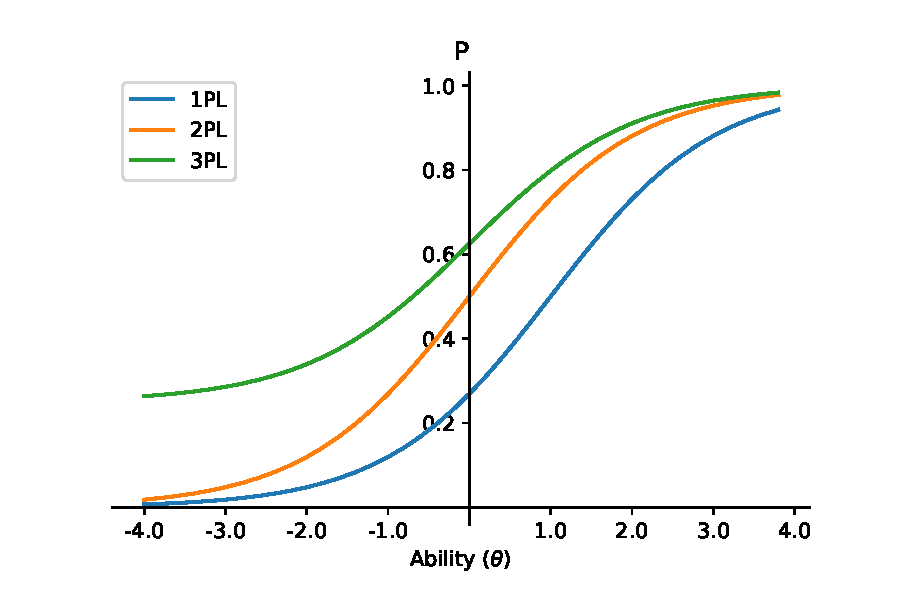
\includegraphics[scale=0.5]{figs/ICC_plots.pdf}
        \end{center}
        \caption{Một ví dụ về chèn hình ảnh.}
        \label{icc_plot}
    \end{figure}
\end{center}

\section{Chèn bảng}

\begin{center}
    \begin{table}
        \centering
        \caption{Ví dụ về tạo bảng trong \LaTeX. Tham khảo: \url{https://en.wikibooks.org/wiki/LaTeX/Tables}.}
        \begin{tabular}{ |l|l|l| }
            \hline
            \multicolumn{3}{ |c| }{Danh sách U23 Việt Nam tại Sea Games 31} \\
            \hline
            Thủ môn                   & GK & Nguyễn Văn Toản                \\ \hline
            \multirow{4}{*}{Hậu vệ}   & LB & Phan Tuấn Tài                  \\
                                      & DC & Bùi Hoàng Việt Anh             \\
                                      & DC & Lê Văn Đô                      \\
                                      & RB & Lê Văn Xuân                    \\ \hline
            \multirow{3}{*}{Tiền vệ}  & MC & Đỗ Hùng Dũng                   \\
                                      & MC & Nguyễn Hoàng Đức               \\
                                      & MC & Dụng Quang Nho                 \\ \hline

            \multirow{2}{*}{Tiền đạo} & ST & Nhâm Mạnh Dũng                 \\
                                      & ST & Nguyễn Văn Tùng                \\
                                      & FW & Nguyễn Tiến Linh               \\
            \hline
        \end{tabular}

    \end{table}
\end{center}

\section{Chèn công thức toán học}

Công thức \ref{eq:InterTweetInteraction} thể hiện mức độ tương tác giữa hai tập $T_{j}^{P}$ và $T_{k}^{P}$.

\begin{align}
    S_{j,k}^{P}=\frac{\sum_{t_{m}^{P}\in T_{j}^{P}}\sum_{t_{n}^{P}\in T_{k}^{P}}r\left(t_{m}^{P},t_{n}^{P}\right)}{|T_{j}^{P}||T_{k}^{P}|}\label{eq:InterTweetInteraction}
\end{align}

Để soạn thảo các công thức toán học được dễ dàng hơn, có thể sử dụng một phần mềm hỗ trợ nhập công thức theo dạng What You See Is What You Mean (WYSIWYM), chẳng hạn như \href{https://www.lyx.org/}{LyX}, sau đó copy LaTeX code vào file .tex (xem Hình \ref{lyx_example}), sẽ được kết quả như Công thức \ref{eq:ErrorFunction}.

\begin{center}
    \begin{figure}[h!]
        \begin{center}
            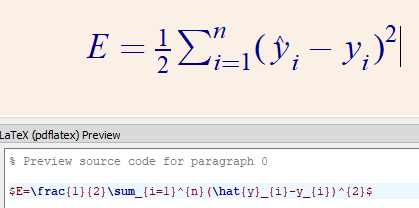
\includegraphics[scale=0.5]{figs/LyX.PNG}
        \end{center}
        \caption{Ví dụ cách soạn thảo công thức bằng LyX và copy sang file .tex.}
        \label{lyx_example}
    \end{figure}
\end{center}

\begin{align}
    E=\frac{1}{2}\sum_{i=1}^{n}(\hat{y}_{i}-y_{i})^{2}
    \label{eq:ErrorFunction}
\end{align}



\section{Chèn mã nguồn}
Có thể sử dụng package minted để chèn mã nguồn vào báo cáo. Có thể chèn mã nguồn trực tiếp hoặc từ file có sẵn.

\noindent\textbf{Ví dụ 1:} Chèn mã nguồn trực tiếp.
\lstset{language=Python}
\begin{lstlisting}
# Hello world program in Python
import math
def solve(a, b, c):
    if a == 0:
        if b != 0:
            return -c/b
        else:
            return "Phuong trinh vo nghiem hoac vo so nghiem"
    else:
        delta = b*b - 4*a*c
        if delta < 0:
            return "Phuong trinh vo nghiem"
        else:
            x1 = (-b + math.sqrt(delta)) / (2*a)
            x2 = (-b - math.sqrt(delta)) / (2*a)
            return x1, x2

print(solve(1, 2, 1))
\end{lstlisting}

\noindent\textbf{Ví dụ 2:} Chèn mã nguồn từ file. Đoạn mã nguồn sau đây được chèn từ file \path{code/XulyFileText.cpp}

\lstinputlisting[language=c++]{code/XulyFileText.cpp}

\section{Biểu diễn giải thuật}
\begin{algorithm}[H]
    \SetAlgoLined
    \KwIn{Hệ số $a$, $b$, và $c$ của phương trình bậc hai $ax^2 + bx + c = 0$}
    \KwOut{Nghiệm của phương trình}
    \If{$a = 0$}{
        \eIf{$b \neq 0$}{
            \Return{$x = -c/b$}\;
        }{
            \Return{Phương trình vô nghiệm hoặc vô số nghiệm}\;
        }
    }
    \Else{
        \textbf{Calculate} $\Delta = b^2 - 4ac$\;
        \eIf{$\Delta < 0$}{
            \Return{Phương trình vô nghiệm}\;
        }{
            \textbf{Calculate} $x1 = (-b + \sqrt{\Delta}) / (2a)$\;
            \textbf{Calculate} $x2 = (-b - \sqrt{\Delta}) / (2a)$\;
            \Return{$x1, x2$}\;
        }
    }
    \caption{Giải thuật giải phương trình bậc hai}
\end{algorithm}



\section{Chèn chú thích vào cuối trang (footnote)}
Khi cần chèn một dòng chú thích vào cuối trang, sử dụng lệnh \textbf{footnote}\footnote{Đây là dòng chú thích}.




\section{Chèn tài liệu tham khảo}

Có thể chèn tài liệu tham khảo vào báo cáo bằng cách sử dụng lệnh \textbf{cite} \cite{DBLP:journals/corr/abs-1908-10084}.
VD: \cite{DBLP:journals/corr/abs-1908-10084}.

VD2: \cite{van2010documentation, Gu_recognitionusing}.

\chapter{Kết luận }\label{chapter_conclusion}

\section{Đánh giá chung về đề tài}
\subsection{Những kết quả đạt được}
\subsection{Một số hạn chế của đề tài}
\section{Hướng phát triển của đề tài}

% Tài liệu tham khảo
\bibliographystyle{plain} 
\bibliography{refs}

% Kết thúc
\end{document}